% Options for packages loaded elsewhere
\PassOptionsToPackage{unicode}{hyperref}
\PassOptionsToPackage{hyphens}{url}
%
\documentclass[
]{article}
\usepackage{amsmath,amssymb}
\usepackage{iftex}
\ifPDFTeX
  \usepackage[T1]{fontenc}
  \usepackage[utf8]{inputenc}
  \usepackage{textcomp} % provide euro and other symbols
\else % if luatex or xetex
  \usepackage{unicode-math} % this also loads fontspec
  \defaultfontfeatures{Scale=MatchLowercase}
  \defaultfontfeatures[\rmfamily]{Ligatures=TeX,Scale=1}
\fi
\usepackage{lmodern}
\ifPDFTeX\else
  % xetex/luatex font selection
\fi
% Use upquote if available, for straight quotes in verbatim environments
\IfFileExists{upquote.sty}{\usepackage{upquote}}{}
\IfFileExists{microtype.sty}{% use microtype if available
  \usepackage[]{microtype}
  \UseMicrotypeSet[protrusion]{basicmath} % disable protrusion for tt fonts
}{}
\makeatletter
\@ifundefined{KOMAClassName}{% if non-KOMA class
  \IfFileExists{parskip.sty}{%
    \usepackage{parskip}
  }{% else
    \setlength{\parindent}{0pt}
    \setlength{\parskip}{6pt plus 2pt minus 1pt}}
}{% if KOMA class
  \KOMAoptions{parskip=half}}
\makeatother
\usepackage{xcolor}
\usepackage[margin=1in]{geometry}
\usepackage{longtable,booktabs,array}
\usepackage{calc} % for calculating minipage widths
% Correct order of tables after \paragraph or \subparagraph
\usepackage{etoolbox}
\makeatletter
\patchcmd\longtable{\par}{\if@noskipsec\mbox{}\fi\par}{}{}
\makeatother
% Allow footnotes in longtable head/foot
\IfFileExists{footnotehyper.sty}{\usepackage{footnotehyper}}{\usepackage{footnote}}
\makesavenoteenv{longtable}
\usepackage{graphicx}
\makeatletter
\def\maxwidth{\ifdim\Gin@nat@width>\linewidth\linewidth\else\Gin@nat@width\fi}
\def\maxheight{\ifdim\Gin@nat@height>\textheight\textheight\else\Gin@nat@height\fi}
\makeatother
% Scale images if necessary, so that they will not overflow the page
% margins by default, and it is still possible to overwrite the defaults
% using explicit options in \includegraphics[width, height, ...]{}
\setkeys{Gin}{width=\maxwidth,height=\maxheight,keepaspectratio}
% Set default figure placement to htbp
\makeatletter
\def\fps@figure{htbp}
\makeatother
\setlength{\emergencystretch}{3em} % prevent overfull lines
\providecommand{\tightlist}{%
  \setlength{\itemsep}{0pt}\setlength{\parskip}{0pt}}
\setcounter{secnumdepth}{5}
\ifLuaTeX
\usepackage[bidi=basic]{babel}
\else
\usepackage[bidi=default]{babel}
\fi
\babelprovide[main,import]{spanish}
% get rid of language-specific shorthands (see #6817):
\let\LanguageShortHands\languageshorthands
\def\languageshorthands#1{}
\usepackage{float}
\usepackage{booktabs}
\usepackage{longtable}
\usepackage{array}
\usepackage{multirow}
\usepackage{wrapfig}
\usepackage{float}
\usepackage{colortbl}
\usepackage{pdflscape}
\usepackage{tabu}
\usepackage{threeparttable}
\usepackage{threeparttablex}
\usepackage[normalem]{ulem}
\usepackage{makecell}
\usepackage{xcolor}
\ifLuaTeX
  \usepackage{selnolig}  % disable illegal ligatures
\fi
\usepackage{bookmark}
\IfFileExists{xurl.sty}{\usepackage{xurl}}{} % add URL line breaks if available
\urlstyle{same}
\hypersetup{
  pdftitle={Análisis de Tickets de Supermercado: Mini Proyecto 2025},
  pdflang={es-ES},
  hidelinks,
  pdfcreator={LaTeX via pandoc}}

\title{Análisis de Tickets de Supermercado: Mini Proyecto 2025}
\usepackage{etoolbox}
\makeatletter
\providecommand{\subtitle}[1]{% add subtitle to \maketitle
  \apptocmd{\@title}{\par {\large #1 \par}}{}{}
}
\makeatother
\subtitle{Tratamiento de datos. Grado en Ciencia de Datos - UV}
\author{}
\date{\vspace{-2.5em}2025-05-06}

\begin{document}
\maketitle

\[\text{Neus Ferrer Font, Marta Navarro García, Alba Rodríguez Simón, Mohammed Aissa Djellouli}\]
\[\text{Héctor Balbastre Aparisi, Joan Ruiz Ripoll, Carlos Santiago Martinez Torres}\]

\section{Introducción}\label{introducciuxf3n}

En este proyecto se plantea realizar el análisis de tickets del supermercado Mercadona, los cuales fueron recolectados por los estudiantes del grado de Ciencia de datos y otros de cursos anteriores.

\subsection{Contexto}\label{contexto}

Actualmente, las grandes empresas gestionan volúmenes significativos de productos, lo que conlleva elevados costes asociados al transporte y almacenamiento. Por este motivo, resulta fundamental optimizar cada etapa del proceso logístico. Con base en nuestro conocimiento en Big Data, nuestro equipo se enfocará en analizar y comprender las tendencias de los consumidores, con el objetivo de reducir costes operativos.

\subsection{Grupo}\label{grupo}

Nuestro objetivo al responder estas preguntas es profundizar en los hábitos y preferencias reales de los consumidores a partir del análisis de tickets de compra. Al extraer patrones y correlaciones dentro de estos datos, buscamos generar conocimiento útil para anticipar comportamientos, mejorar la planificación comercial y ajustar la oferta a la demanda real. Esta aproximación nos permitirá aportar valor estratégico desde el análisis de datos, con el foco puesto en reducir ineficiencias, mejorar la toma de decisiones y apoyar la sostenibilidad operativa del negocio desde una perspectiva basada en la evidencia.

\subsection{Preguntas planteadas}\label{preguntas-planteadas}

1)¿Qué frutas tienen mayor venta en primavera?

2)¿Qué eventos locales o festivos generan picos de venta significativos? (Ej. Navidad)

3)¿Existen diferencias significativas en las preferencias de compra según zonas (urbana vs rural)?

4)¿Qué categorías tienen mayor tendencia a generar compras adicionales (por ejemplo, comprar galletas con café)?

5)¿Qué productos muestran mayor consistencia de compra independientemente de cambios en su precio?

6)¿Cuántos productos compra en promedio una persona por ticket?

7)¿Cuál es el gasto promedio por compra y Cómo varía según el día/hora?

8)¿Qué categorías de productos (fruta, verdura\ldots{} )suelen comprarse juntas con mayor frecuencia?

9)¿Hay diferencias de consumo en días laborales vs.~fines de semana?

10)¿Cuál es el mejor horario para comprar? (Menos concurrencia)

11)¿Cuál es el mejor día para comprar? (Menos concurrencia)

12)¿Qué mes es mejor para comprar x fruta? (El mes con mayor compra de frutas y verduras)

13)¿Cuál ha sido el producto, unitario, más comprado y cuál ha sido el cambio de su precio a lo largo del tiempo?

14)¿Cuáles son los productos con mayor facturación total? (Top 5 de los más facturados)

15)¿Cómo varían las ventas a lo largo del mes? ¿Hay más compras a fin de mes?

16)¿Cuál es la tasa de personas que al comprar, tienen parking? (Compras con parking/Total de compras)

17)¿Qué productos aparecen con mayor frecuencia en los tickets de alto valor (€)?

18)¿Qué combinaciones de productos se repiten con más frecuencia en una misma compra?

\section{Material y métodos}\label{material-y-muxe9todos}

\subsection{Carga de librerias}\label{carga-de-librerias}

Para la carga de librerías, haremos uso del paquete pacman de R, que es eficiente para la carga e instalación de las mismas. En este proyecto, utilizaremos las librerias pdftools, tidyverse, readxl, lubridate, visdat y knit.

\subsection{Carga de datos}\label{carga-de-datos}

Todos nuestros datos están almacenados la carpeta \emph{.data}, y fueron obtenidos desde un repositorio en la nube. Todos los ficheros contenidos en esta carpeta están en formato \emph{.pdf}.

Antes de empezar con la extracción de los datos, fue necesario preguntarse: ¿Qué información queremos almacenar? ¿Cómo vamos a almacenar la información? Adicionalmente, para evitar problemas con la extracción y lectura de datos desde los ficheros \emph{pdf} al entorno de R, se estableció que lo mejor sería tratar todos los datos como caracteres. Una vez que todos los datos fueran leídos correctamente, se podría hacer la conversión al tipo de dato correspondiente.

\emph{Nota:} A lo largo de la extracción de los datos, se implementaron funciones para ser recursivos, además de facilitar la lectura del código y hacer una carga completa (barrido) de los datos contenidos en los ficheros.

Dentro de cada fichero, encontramos dos partes fundamentales. La primera, es el encabezado. Contiene información sobre la compra en general. Por ejemplo, reune datos como la ubicación de la tienda, fecha y hora de compra, y número de ticket. En la segunda parte, nos encontramos con el bloque de los productos. En ella se describe el producto comprado, la cantidad y el importe pagado.

Para la lectura de los productos, identificamos dos filtros esenciales. El primero, es si el ticket incluía parking o no. Este `producto' estaba listado al final, lo que nos permitía de alguna forma reducir el listado de productos e identificar si había o no parking.

El segundo filtro, permitía saber si se compró pescado o no. Este filtro fue de gran utilidad dado que por la naturaleza de negocio de Mercadona, los tickets y los productos vienen clasificados en 3 categorías:

\begin{itemize}
\tightlist
\item
  Venta por unidad.
\item
  Venta al peso, pescado.
\item
  Venta al peso, frutas y verduras.
\end{itemize}

Si en el ticket se registró la compra de pescado, ya podíamos establecer que a partir de ese filtro, los productos que estuvieran por debajo de esa línea, serían al peso. Y los que no, serían por unidad. Una vez que se identificara el tipo de producto, unitario o al peso, ya sería más fácil identificar la categoría a la que pertenece, por el formato en que fue registrado el producto en el ticket.

\subsection{Ficheros no leidos}\label{ficheros-no-leidos}

Solo aquellos ficheros que estuvieran con el formato correcto, serían tratados. Es decir, aquellos ficheros que tuvieran un escaner, foto u otro formato de factura distinto al formato de Mercadona, no serían tratados. Para identificarlos y corroborar su contenido, hemos almacenado el nombre del fichero en un dataframe diferente \emph{NoLeido}.

\subsection{Presentación parcial de los datos}\label{presentaciuxf3n-parcial-de-los-datos}

Esta es una representación sobre cómo se almacenaron los datos para empezar a trabajar sobre ellos. En la Tabla \ref{tab:TablaTiendas} podemos ver todas las tiendas en las que se han hecho las compras. En total, se han registrado 35 tiendas.

\begin{table}[!h]
\centering
\caption{\label{tab:TablaTiendas}Tabla de tiendas leidas}
\centering
\resizebox{\ifdim\width>\linewidth\linewidth\else\width\fi}{!}{
\begin{tabular}[t]{lllll}
\toprule
IdTienda & Direccion & CodigoPostal & Municipio & Telefono\\
\midrule
\cellcolor{gray!10}{2916} & \cellcolor{gray!10}{CTRA. GARRUCHA A VERA S/N} & \cellcolor{gray!10}{04630} & \cellcolor{gray!10}{GARRUCHA} & \cellcolor{gray!10}{950133380}\\
2233 & AVDA. VALENCIA 41 & 03830 & MURO & 966516066\\
\cellcolor{gray!10}{4530} & \cellcolor{gray!10}{C/ ALICANTE 83} & \cellcolor{gray!10}{03801} & \cellcolor{gray!10}{ALCOI/ALCOY} & \cellcolor{gray!10}{965366422}\\
3075 & C/ MENORCA (C.C. AQUA) 19 & 46023 & VALENCIA & 963319378\\
\cellcolor{gray!10}{3095} & \cellcolor{gray!10}{C/ VALENCIA S/N} & \cellcolor{gray!10}{03178} & \cellcolor{gray!10}{BENIJOFAR} & \cellcolor{gray!10}{966713008}\\
\addlinespace
4478 & AVDA. DEL TEXTIL 21 & 46870 & ONTINYENT & 961484834\\
\cellcolor{gray!10}{4347} & \cellcolor{gray!10}{C/ PERIODISTA AZZATI 26} & \cellcolor{gray!10}{46520} & \cellcolor{gray!10}{SAGUNT/SAGUNTO} & \cellcolor{gray!10}{961485847}\\
4583 & C/ MANUEL CANDELA 16 & 46021 & VALENCIA & 961624385\\
\cellcolor{gray!10}{3957} & \cellcolor{gray!10}{C/ PINTOR MAELLA 3} & \cellcolor{gray!10}{46023} & \cellcolor{gray!10}{VALENCIA} & \cellcolor{gray!10}{962564516}\\
2473 & AVDA. CARDENAL BENLLOCH 91 & 46021 & VALENCIA & 963612915\\
\bottomrule
\end{tabular}}
\end{table}

En la siguiente Tabla \ref{tab:TablaProductos} se muestran los productos que fueron leídos, identificando por ejemplo el ticket de compra, la fecha, el tipo de producto, entre otros.

\begin{table}[!h]
\centering
\caption{\label{tab:TablaProductos}Tabla de productos leidos}
\centering
\resizebox{\ifdim\width>\linewidth\linewidth\else\width\fi}{!}{
\begin{tabular}[t]{llllllllll}
\toprule
Fecha & IdTienda & IdFactura & Hora & Producto & Cantidad & PrecioUnitario & Importe & TipoProducto & Parking\\
\midrule
\cellcolor{gray!10}{25/11/2023} & \cellcolor{gray!10}{2916} & \cellcolor{gray!10}{520925} & \cellcolor{gray!10}{09:09} & \cellcolor{gray!10}{DONACIÓN} & \cellcolor{gray!10}{5} & \cellcolor{gray!10}{1,00} & \cellcolor{gray!10}{5,00} & \cellcolor{gray!10}{Unitario} & \cellcolor{gray!10}{TRUE}\\
25/11/2023 & 2916 & 520925 & 09:09 & BARREÑO & 1 & 2,20 & 2,20 & Unitario & TRUE\\
\cellcolor{gray!10}{25/11/2023} & \cellcolor{gray!10}{2916} & \cellcolor{gray!10}{520925} & \cellcolor{gray!10}{09:09} & \cellcolor{gray!10}{PALO ANTIDESLIZANTE} & \cellcolor{gray!10}{3} & \cellcolor{gray!10}{1,90} & \cellcolor{gray!10}{5,70} & \cellcolor{gray!10}{Unitario} & \cellcolor{gray!10}{TRUE}\\
25/11/2023 & 2916 & 520925 & 09:09 & MULTIUSOS & 1 & 2,55 & 2,55 & Unitario & TRUE\\
\cellcolor{gray!10}{25/11/2023} & \cellcolor{gray!10}{2916} & \cellcolor{gray!10}{520925} & \cellcolor{gray!10}{09:09} & \cellcolor{gray!10}{AGUA MINERAL} & \cellcolor{gray!10}{2} & \cellcolor{gray!10}{0,73} & \cellcolor{gray!10}{1,46} & \cellcolor{gray!10}{Unitario} & \cellcolor{gray!10}{TRUE}\\
\addlinespace
25/11/2023 & 2916 & 520925 & 09:09 & B.BASURA EXT.C.FÁCIL & 2 & 1,60 & 3,20 & Unitario & TRUE\\
\cellcolor{gray!10}{25/11/2023} & \cellcolor{gray!10}{2916} & \cellcolor{gray!10}{520925} & \cellcolor{gray!10}{09:09} & \cellcolor{gray!10}{ESCURRE FÁCIL} & \cellcolor{gray!10}{1} & \cellcolor{gray!10}{2,85} & \cellcolor{gray!10}{2,85} & \cellcolor{gray!10}{Unitario} & \cellcolor{gray!10}{TRUE}\\
25/11/2023 & 2916 & 520925 & 09:09 & CUBO FREGAR C/RUEDAS & 1 & 3,85 & 3,85 & Unitario & TRUE\\
\cellcolor{gray!10}{25/11/2023} & \cellcolor{gray!10}{2916} & \cellcolor{gray!10}{520925} & \cellcolor{gray!10}{09:09} & \cellcolor{gray!10}{FRIEGASUELOS PINO} & \cellcolor{gray!10}{1} & \cellcolor{gray!10}{0,95} & \cellcolor{gray!10}{0,95} & \cellcolor{gray!10}{Unitario} & \cellcolor{gray!10}{TRUE}\\
25/11/2023 & 2916 & 520925 & 09:09 & FIBRAS CRUZADAS & 2 & 2,10 & 4,20 & Unitario & TRUE\\
\bottomrule
\end{tabular}}
\end{table}

\section{Limpieza de datos}\label{limpieza-de-datos}

Para garantizar la fiabilidad de los datos y realizar su posterior análisis, es importante realizar el proceso de limpieza de datos. Podremos ver los valores NA, máximos, mínimos, y evaluar las diferentes características.

\subsection{Valores vacios}\label{valores-vacios}

En principio, dada la naturaleza del ejercicio, de extracción y carga de los datos, no deberían haber valores nulos. Sin embargo, es necesario verificar, especialmente con los dataframes que queremos analizar: Compra y Tienda.

\subsection{Problemas con tipos de datos}\label{problemas-con-tipos-de-datos}

Vamos a hacer usar \emph{glimpse} de los dataframes para comprobar que cada columna tenga su tipo adecuado. En el dataframe de tienda, podriamos poner tanto el id, el codigo postal, y el telefono como números enteros, pero, ya que no tendria sentido realizar operaciones propias de los numeros enteros con estos datos, no será necesario.

Ahora bien, con el dataframe Compra no podemos hacer lo mismo. Las variables de Fecha y Hora deberán ser tratadas como `tiempo'. Cantidad, precio unitario e importe deberian ser de tipo numérico; es importante sustituir las comas por puntos para identifical los decimales y transformar correctamente el dato. Por último, el tipo de producto y la variable parking, que serán de tipo categórico.

Para finalizar hacemos una verificacion sobre los valores repetidos. En principio, no deberían haber valores repetidos, ya que al hacer el registro de los datos, se evito este problema. Sin embargo, usando \emph{unique} podemos asegurarnos.

\section{Resultados}\label{resultados}

\subsection{Análisis de varibales}\label{anuxe1lisis-de-varibales}

Por la naturaleza de los datos y la manera en que se desarollará el trabajo, abordaremos el análisis de las variables categóricas como \emph{TipoProducto} y \emph{Parking}, y de tipo fecha posteriormente, dentro de nuestro dataframe de Compras.

\begin{verbatim}
## Rows: 4,807
## Columns: 10
## $ Fecha          <date> 2023-11-25, 2023-11-25, 2023-11-25, 2023-11-25, 2023-1~
## $ IdTienda       <chr> "2916", "2916", "2916", "2916", "2916", "2916", "2916",~
## $ IdFactura      <chr> "520925", "520925", "520925", "520925", "520925", "5209~
## $ Hora           <Period> 9H 9M 0S, 9H 9M 0S, 9H 9M 0S, 9H 9M 0S, 9H 9M 0S, 9H~
## $ Producto       <chr> "DONACIÓN", "BARREÑO", "PALO ANTIDESLIZANTE", "MULTIUSO~
## $ Cantidad       <dbl> 5, 1, 3, 1, 2, 2, 1, 1, 1, 2, 1, 1, 1, 1, 1, 1, 1, 1, 1~
## $ PrecioUnitario <dbl> 1.00, 2.20, 1.90, 2.55, 0.73, 1.60, 2.85, 3.85, 0.95, 2~
## $ Importe        <dbl> 5.00, 2.20, 5.70, 2.55, 1.46, 3.20, 2.85, 3.85, 0.95, 4~
## $ TipoProducto   <fct> Unitario, Unitario, Unitario, Unitario, Unitario, Unita~
## $ Parking        <fct> TRUE, TRUE, TRUE, TRUE, TRUE, TRUE, TRUE, TRUE, TRUE, T~
\end{verbatim}

Sin embargo, para familiarizarnos con los datos, analizaremos los precios medios de los productos, dado que han variado a lo largo del tiempo, y las palabras que más se repiten en la descripción de los productos (Figura \ref{fig:FiguraPalabras}). En nuestro estudio encontramos dos variables numéricas que se encuentran en el dataframe de los productos comprados. Realizando el análisis sobre la variable \emph{PrecioUnitario}, vemos su distribución en el gráfico \ref{fig:FiguraPrecios}, donde la mayoría de los precios promedio de Mercadona no superan los 10 EUR. Sin embargo, considerando la detección por la regla de boxplot, ya que no se sigue una distribución normal, aquellos valores por debajo de 1.4 y por arriba de 3.12 son consideros como outliers.

\begin{figure}[H]

{\centering 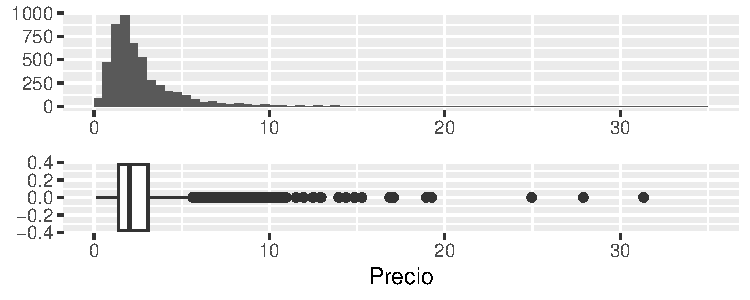
\includegraphics{ProyectoTD2025_files/figure-latex/FiguraPrecios-1} 

}

\caption{Distribución de los precios}\label{fig:FiguraPrecios}
\end{figure}

\begin{figure}

{\centering 
\includegraphics{ProyectoTD2025_files/figure-latex/FiguraPalabras-1} 

}

\caption{Nube de palabras de productos}\label{fig:FiguraPalabras}
\end{figure}

\subsection{Continuación análisis\ldots{}}\label{continuaciuxf3n-anuxe1lisis}

\section{Conclusiones}\label{conclusiones}

\end{document}
